In this module you will learn
\begin{itemize}
	\item how to model two or more inter-dependent quantities using systems
\end{itemize}

\hfill \\


Often, when modelling something, we are faced with two or more quantities that depend on each other. This means that one equation is not enough, so we need to learn how to deal with a system of equations. \\


Just like we did in module \ref{model-odes}, we will follow the step by step procedure developed in chapter 1.

\paragraph{\emph{Step 1.}} Define the problem

\begin{example}
We want to model two interacting populations, like the populations of bears and salmon in a specific natural park.\\

The first step is to decide on what we want to find at the end of the process. 
In this case, we want to know the number of individuals in each population and how they change as time passes. So we define:
\begin{itemize}
	\item $b(t) =$ number of bears in the natural park at time $t$;
	\item $s(t) =$ number of salmon in the natural park at time $t$.
\end{itemize}
\end{example}


\paragraph{\emph{Step 2.}} Build a mind map

\begin{example}
We start with both species in the centre:

\def\SalmonBear{
	\fill[color=orange!50!white] (-4,0) rectangle (-2,1) node[pos=.5] {\color{black}Salmon};
	\fill[color=brown!60!white] (4,0) rectangle (2,1) node[pos=.5] {\color{black}Bear};
}
\begin{center}
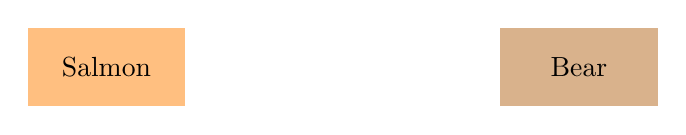
\begin{tikzpicture}
	\SalmonBear
\end{tikzpicture}
\end{center}

We can start brainstorming about the things that affect these populations:
\begin{center}
%\begin{tikzpicture}
%	\SalmonBear
%    \begin{scope}[decoration={
%    markings,
%    mark=at position 0.5 with {\arrow{>}}}
%    ]
%	\draw[postaction={decorate}] (-2,1) arc (120:60:4) node[pos=0.5,above] {food};
%    \draw[postaction={decorate}] (2,0) arc (300:240:4) node[pos=0.5,below] {hunts};
%    \end{scope}
%    \draw (-3,0) -- (-4,-1);
%    \fill[color=green!50!white] (-5.25,-2) rectangle (-2.75,-1) node[pos=.5] {\color{black}reproduction};
%    \draw (-3,1) -- (-4,2);
%    \fill[color=yellow!50!white] (-5.25,2) rectangle (-2.75,3) node[pos=.5] {\color{black}habitat limits};
%    \draw (3,0) -- (4,-1);
%    \fill[color=red!50!white] (5.25,-2) rectangle (2.75,-1) node[pos=.5] {\color{black}competition};
%    \draw (3,1) -- (4,2);
%    \fill[color=yellow!50!white] (5.25,2) rectangle (2.75,3) node[pos=.5] {\color{black}habitat limits};
%\end{tikzpicture}
\begin{tikzpicture}
	\SalmonBear
    \begin{scope}[decoration={
    markings,
    mark=at position 0.5 with {\arrow{>}}}
    ]
    \draw[postaction={decorate}] (-2,0.5) -- (2,0.5) node[pos=0.5,above] {food};
    \draw[postaction={decorate}] (2,0) arc (300:240:4) node[pos=0.5,below] {hunts};
    \end{scope}
    \draw (-3,0) -- (-4,-1);
    \fill[color=green!50!white] (-5.25,-2) rectangle (-2.75,-1) node[pos=.5] {\color{black}reproduction};
    \draw (-3,1) -- (-0.5,2);
    \draw (3,1) -- (0.5,2);
    \fill[color=yellow!50!white] (-1.5,2) rectangle (1.5,3) node[pos=.5] {\color{black}habitat limits};
    \draw (3,0) -- (4,-1);
    \fill[color=red!50!white] (5.25,-2) rectangle (2.75,-1) node[pos=.5] {\color{black}competition};
\end{tikzpicture}
\end{center}
	
\end{example}


\paragraph{\emph{Step 3.}} Make assumptions

\begin{example}
In this step, we discuss which of the boxes in the mind map we want to actually consider in our model, and which assumptions we need to make to consider them. \\

Let us start with how these species interact with each other:
\begin{enumerate}
	\item Salmon provide food for bears: the bear population profits from each encounter with salmon. How does each bear-salmon encounter affect the bear population?
	\item Bears hunt salmon: the salmon population is likely to decrease with each encounter with a bear. How does each bear-salmon encounter affect the salmon population?
\end{enumerate}

These two components are essential in our model, so we need to include them. It still leaves some freedom on how to do this. \\

There are other elements that we might want to include in our model:
\begin{enumerate}[start=3]
	\item Salmon reproduction: in the absence of predators and under ideal conditions, salmon should grow according to the Malthusian model, i.e. the rate of growth is proportional to the number of salmon;
	\item Bear competition: bears are mainly predators, so without salmon, their numbers will decrease, also according to the Malthusian model;
	\item Habitat limits: these species live in habitats that have limited resources, so we can consider a carrying capacity for each species.
\end{enumerate}

To make the model simpler, we will \emph{ignore habitat limits}. This means that this model will not be accurate if the populations become very large.
	
\end{example}


\paragraph{\emph{Step 4.}} Construct a model

\begin{example}
We will start with our populations:
\begin{itemize}
	\item $b(t)$
	\item $s(t)$
\end{itemize}
and we will start adding components to each of these one by one. \\

For the first two items, we need to estimate the number of encounters salmon-bear. We assume that the number of encounters is proportional to the number of all possible encounters: \emph{$b(t)\, s(t)$}.

\begin{enumerate}
	\item Salmon provide food for bears: for every possible salmon-bear encounter, there is a probability that a bear actually encounters a salmon, and then there is a chance that the bear will catch the salmon. Each catch improves the possibility that the bear population will increase. All these put together means that this factor should increase the bear growth rate by \emph{$a \,b(t)\, s(t)$}, where the constant $a$ needs to be found.
	\item Bears hunt salmon: similarly to the previous item, for every possible encounter, there is a probability that the bear actually encounters a salmon, and then there is a chance that the bear will catch the salmon. Every catch will decrease the salmon population, so the salmon growth rate will decrease by \emph{$c \,b(t) \,s(t)$}, there the constant $b$ needs to be found.
\end{enumerate}

Right now we have the following model:
$$
\begin{cases}
b'(t) = a \,b(t)\, s(t) + \cdots \\
s'(t) = - c \,b(t)\, s(t) + \cdots	
\end{cases}
$$

We continue with the other elements:
\begin{enumerate}[start=3]
	\item Salmon reproduction: this was explained before and should contribute to the salmon growth rate with the term \emph{$d s(t)$}.
	\item Bear competition: this was also explained above and should contribute to the bear growth rate with the term \emph{$-e b(t)$}.
	\item Habitat limits: we decided to ignore this.
\end{enumerate}

We have the model:
$$
\begin{cases}
b'(t) = a \, b(t) \,s(t) -e \, b(t) \\
s'(t) = - c \, b(t) \,s(t) + d \, s(t)
\end{cases}
$$

To find the constants $a,c,d,e$, we would probably need to go back to Step 3 and make further assumptions related to the way that we are measuring them.
\end{example}



\paragraph{\emph{Step 5.}} Model assessment

\begin{example}

We can do several things here. I'll let you brainstorm and think of ways you can assess this model.

One of the things that we can do is approximate its solutions using Euler's Method discussed in Module \ref{Approximation}. 

Let us assume, for this example the constants: $a=1$, $e=10$, $c=1$, $d=5$ and a time step $\Delta t = 0.5$ and we assumed an initial population of $b(0)=6$ and $s(0)=9$. Then we obtain the graph below:


\begin{center}
\includegraphics*[width=200pt]{images/module15-lotka-volterra.png}
\end{center}
\begin{itemize}
	\item \url{https://www.desmos.com/calculator/zywspwstwk} \hfill \qrcode{https://www.desmos.com/calculator/zywspwstwk}
\end{itemize}

The $x-$axis is the bear population while the $y-$axis is the salmon population. Each dot gives gives an approximation of the populations $\Delta t = 0.5$ time units after the previous approximation.\\


From this approximation, we can say infer that this model creates a population cycle, but it seems to spiral outwards: 
\begin{center}
\includegraphics*[width=200pt]{images/module15-lotka-volterra-more.png}
\end{center}

\begin{itemize}
	\item Is having a population cycle a feature that our model should have?
	\item Is the spiralling outwards a feature we want in our model?
	\item Is the spiralling a feature of the model or the approximation? If it's from the approximation, how does the model behave?
\end{itemize}

\end{example}



\paragraph{\emph{Step 6.}} Putting it all together in a report

We'll skip this part here.




